\documentclass[a4paper,12pt]{article}
\usepackage[english]{babel}
\usepackage{mathtools}
\usepackage{graphicx}
\usepackage[utf8]{inputenc}
\graphicspath{ {graphs/} }

\begin{document}

\title{Force Directed Graph Drawing algorithms\\ \bigskip \large{Group Charlie-5}}
\author{Jeroen Hoegen Dijkhof \and Roxanne Giling \and Laurens Post}
\maketitle
\begin{abstract}
Force-directed graph drawing is a useful method to display graphs in an ordered and readable way. In this paper we will describe our analysis of the impact of several variables of the Eades algorithm and compare its runtime and practical time complexity with the Fruchterman and Reingold algorithm.
\end{abstract}
\newpage

\section{Introduction}\label{s:Introduction}
A graph as we know it in the world of computer science consists of a set of vertices (more commonly referred to as nodes) and a set of edges connecting these vertices\cite{Graph}. A graph can be used to represent several things, ranging from relationships between friends to connections between servers and their clients. Humans are able to draw such a graph on paper while making it easy and intuitive to read without many difficulties. For a computer, this is not as simple and thus there exists various algorithms which attempt to achieve this. A well known method is Force-directed graph drawing. It has been one of the most flexible and widely used algorithms since its invention in 1963, with one of the first versions being that of ~Tutte~\cite{Tutte}. These algorithms attempt to represent graphs in an aesthetically pleasing way. This is done by spacing out the vertices from each other (they must be clearly visible as separate vertices), but keeping related vertices together and attempting to reduce the total area covered by the resulting image. The algorithms are based on the idea of physical springs and magnets in that each vertex has both a repulsive as well as an attractive force pulling and pushing on them. Ideally, this makes two vertices spaced out in such a way that these two forces are in balance with each other. As a graph grows in size, so does its complexity. Lines may cross with one another or connected vertices may find themselves stretched out on either side of the initial graph. In our research we have discovered a variety of algoritms, each with their own ideas on how to compute these two forces and how to handle this increase in complexity. Tutte, as mentioned above, uses a graph's Barycentric representation while others, such as that of Kamada and ~Kawai~\cite{Kawai}, use the theoretic distances of paths in the graph from one vertex to another in order to compute their spring forces. We have gotten most of our information from Kobourov\cite{Kobourov}, including the algorithm that we ended up using as described below in section \ref{s:algorithm}.

\section{Research question}\label{s:question}
Eades' 1984 algorithm\cite{Eades} is relatively easy to implement, but the paper mentions limits to it's suitability for larger data sets and notes several predetermined constants. A lot has changed in computer science since 1984. Our research question is thus as follows: Is the research done for the Eades algorithm still relevant to today's standard in technology? In order to answer this question we have divided this question up into sub-questions:
\begin{itemize}
\item What happens if we change up some of the constants of the algorithm?
\item What happens when we increase the number of vertices in the graph?
\item How does this behaviour compare to other algorithms?
\end{itemize}

\section{Description of the experiments}
As stated above, a wide variety of algoritms exist. To clarify exactly which variant we will study, we shall first describe what we used exactly, how we used it and what kinds of results we wanted to receive as output data.
\subsection{Eades' Algorithm}\label{s:algorithm}
For our research, we implemented the relatively simple Spring algorithm designed by Eades in the C\# language. It is an algorithm designed to be used on graphs consisting of at most 30 vertices. The idea of this algorithm is that each vertex starts out in a randomised position in the field. Then it loops through the list of vertices and adds a certain amount of force to each vertex. This force, recalculated with every new iteration, moves the vertex around. To calculate this force, one first loops over every other vertex in the graph. For every neighbouring vertex (the ones connected to the current vertex by an edge), we calculate an attracting force. These edges try to contract and pull the vertices closer together. This spring force is based on Hookes Law\cite{Hooke} which states that spring force is dependent on distance. For every non-neighbouring vertex we calculate a repelling force. These vertices try to get away from each-other. This results in a tug-of-war between vertices.
\newline
The attractive force is calculated by the following equation:
\begin{equation}\label{e:attract}
f_a = c_1*log(\frac{d}{c_2})
\end{equation}
In this equation, \emph{d} is the length of the edge between the current vertex and its neighbouring vertex that we are looking it and \emph{$c_1$} and \emph{$c_2$} are constants. Note that there is no need to have a repelling force between two vertices connected by an edge, as the springs will repel when over-compressed, i.e., when $d < c_2$.
\newline
The repelling force is calculated by the following equation:
\begin{equation}\label{e:repel}
f_r = \frac{c_3}{d^2}
\end{equation}
Once again, \emph{d} is the distance between the pair of vertices we are currently looking at and \emph{$c_3$} is a constant. With these two equations in place, we can see that the logarithmic attractive force stands opposite the quadratic repelling force. This should in theory result in a graph where these two forces are balanced with each-other.
\newline
After we have calculated all forces that apply to the current vertex using equations \ref{e:attract} and \ref{e:repel}, we add them all up and we are left with a vector that pushes a vertex in a certain direction with a certain velocity, depending on the outcome. This result however may be too strong and so we add a final equation.
\begin{equation}\label{e:damper}
f_{final} = c_4 * f_{results}
\end{equation}
$c_4$ is once again a predefined constant. This is put in place to make sure that the vertices don't move too chaotically which may result in distorted graphs or it could heavily increase the time it takes until the graph stabilizes.
\newline
According to Eades, research has shown that the values $c_1=2$, $c_2=c_3=1$ and $c_4=0.1$ give the best results for most input graphs and that almost all graphs stabilize with $M=100$ where \emph{M} is the number of iterations.
\newline
An analysis of this algorithm shows that every iteration of the algorithm computes the attractive forces in $O(|E|)$ time where \emph{E} is the collection of edges in the graph since it has to look at every edge in the graph only once in order to calculate the spring forces for both connected vertices. The repulsive forces are calculated between all pairs of vertices and as such, the time it takes to compute this is $O(|V|^2)$ where \emph{V} is the collection of all vertices. The iterations are run \emph{M} times and so the time complexity of the algorithm is defined as $O(M*(|E| + |V|^2))$.
\subsection{Fruchterman and Reingold}
As part of our experiment, we also found an extension to the above algorithm designed by Fruchterman and Reingold\cite{FandR}. We wanted to see optimised this version of the algorithm is relationship to that of Eades. This extension redefines equations \ref{e:attract} and \ref{e:repel} as follows:
\begin{equation}\label{e:FRattract}
f_a(d)=\frac{d^2}{k}
\end{equation}
\begin{equation}\label{e:FRrepel}
f_r(d)=\frac{k^2}{d}
\end{equation}
much like in the previous versions of these equations, \emph{d} is once again the distance between the pair of vertices currently looked at. The variable \emph{k} is defined as the optimal distance between the two vertices within the current graph. It is calculated as follows:
\begin{equation}\label{e:optimalD}
k=C*\sqrt{\frac{A}{|V|}}
\end{equation}
In this new equation, \emph{A} is the total area of the graph and \emph{V} is the collection of vertices within the graph. \emph{C} is defined as the temperature of the graph. Fruchterman and Reingold describe this as a way to control the displacement of vertices. If the graph is highly suboptimal, the temperature is high and this allows the vertices to keep moving. As the graph layout approaches an optimal layout, this temperature is decreased and as such, the vertices move slower and slower until they eventually come to a complete stand still. This approach is based on the idea of simulated annealing.
\newline
This extension of the Spring algorithm increases the number of vertices allowed in a graph up to 40, but this is still a very small amount. The time complexity of the algorithm stays the same as with Eades. It is important to note that the time complexity of the repulsive forces can be decreased by only looking at nearby vertices rather than all vertices in the graph. We did not implement this in our project.
\subsection{Test data}
We have generated our own graphs as input data with sizes 4, 8 and 16 vertices and with several different set-ups of edges. Each of these graphs are two-dimensional and undirected. We have also decided to use graphs from an internet database. These we could not describe here since they are fairly large and would take too much time for us to sift through it all. The database can be found here\cite{Database}.
\subsection{Output data}
As output data, we get optimised graphs of course, but in order to answer our subquestions, we wanted more than just that. As such, we have added in a Stopwatch in order to measure the runtime. Since the stopwatch class in C\# is dependent on the pc that it is run on, we can never truly be exact. Thus we execute the program on a given graph several times and take the average time based on the results.Furthermore, we take into consideration the average edge-length and the number of iterations until stabilization.

\section{Results}\label{s:results}
Our results were interesting and proved some of our hypotheses right while proving others wrong. We continuously used 5 tests per different variable setting.
\begin{itemize}
\item We hypothesised that the runtime of the algorithm increases linearly as the number of iterations increases. This implies that each iteration computes in roughly the same amount of time.
\item We hypothesised that the runtime of the algorithm increases quadratically as the number of input vertices increases. This has been proven mostly true. As shown in the figure below, both F\&R and Eades are a good fit, with Coefficients of Determination above 0.95. Furthermore, a two-tailed, paired-samples t-test shows that the runtime values are clearly unrelated with $p = 3.8 * 10^{-17}$ with $n = 570$. Interestingly, Eades shows $\mathcal{O}(n^3)$-like behaviour, whereas $\mathcal{O}(n^2)$ is expected. F\&R does behave as expected.
\begin{figure}[h]
  \centering
  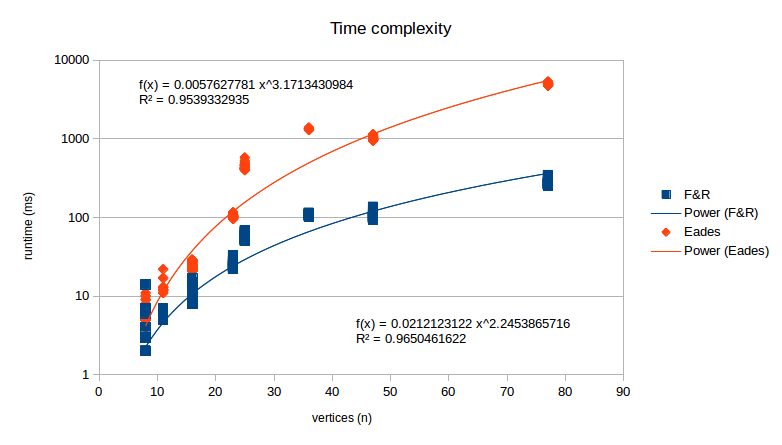
\includegraphics[height=7cm]{timecomplexity}
  \label{fig:timecomplexity}
\end{figure}
\item We hypothesised that the average edge-length decreases linearly as we decrease the value of $c_1$. This was proven wrong however. We found that the mean increased and we calculated the correlation to be $r=-0.73278$ which is a fairly strong negative correlation. As we can see in figure \ref{fig:graphc1}, this increase does not appear to be linear.
\begin{figure}[h]
	\centering
	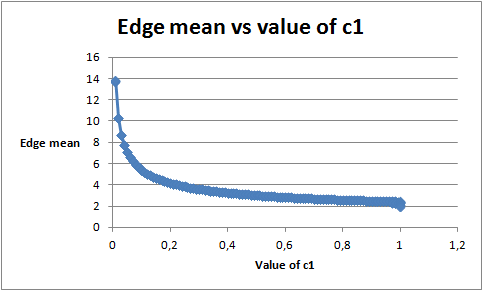
\includegraphics[height=4cm]{Edgemeanvsc1}
	\label{fig:graphc1}
\end{figure}
The resulting graphs became smaller and smaller and as such, became increasingly harder to read. It is also important to note that the standard deviation of the edge-lengths increased as $c_1$ decreased.
\item We hypothesised that the average edge-length increases linearly as we increase the value of $c_3$. The results seem to conform to this. The mean increased and we found the correlation to be $r=0.97092$ which is a very strong positive correlation. As we can see in figure \ref{fig:graphc3}, this increase looks like it forms a nice line with some odd values near the end that we could not explain.
\begin{figure}[h]
	\centering
	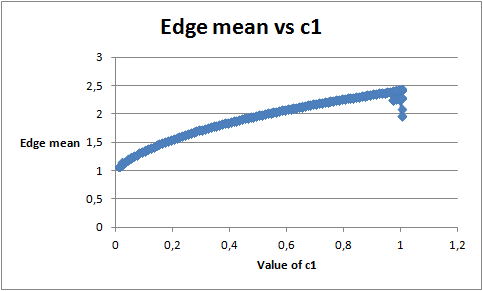
\includegraphics[height=4cm]{Edgemeanvsc3}
	\label{fig:graphc3}
\end{figure}
The resulting graphs became bigger and bigger and as such they became hard to read and put into one image. The standard deviation increased as well.

\item We hypothesised that the run time of the algorithm increases linearly as the amount of simulation iterations increases. This has been proven correct for both the algorithm by Eades and the algorithm by F\&R. We have taken our input values and calculated the correlation between the amount of iterations the simulation has run and the amount of time it took to complete the simulation. The coefficients were as follows:\\
\begin{tabular}{|c|c|}
\hline 
Eades & Fruchtman \& Reingold \\ 
\hline 
0.997829143& 0.998978831 \\ \hline 
0.996927906& 0.995757504 \\ \hline 
0.997490337& 0.997700843 \\ \hline 
0.991544087& 0.9902479 \\ \hline 
0.997503528& 0.996363056 \\ \hline 
0.996257363& 0.994829416 \\ \hline 
0.999352504& 0.999482967 \\ \hline 
0.997158802& 0.994987758 \\ \hline 
0.993337222& 0.988891881 \\ \hline 
0.998740259& 0.999288263 \\ \hline 
0.997058942& 0.995596278 \\ \hline 
0.998111649& 0.996363793 \\ \hline 
0.998624186& 0.996538702 \\ \hline 
0.996166923& 0.998535299 \\ \hline 
0.999083811& 0.998397619 \\ \hline 
0.997805027& 0.996253847 \\ \hline 
0.99772634& 0.990304551 \\ \hline 
0.998800511& 0.997882872 \\ \hline 
0.999360905& 0.998293157 \\ \hline 
0.9986418& 0.998688101 \\ \hline 
\end{tabular} 
The average correlation coefficient for the Eades algorithm was $0.997376062$. For F\&R, this value was $0.996169132$.
\end{itemize}

\section{Discussion and conclusion}
In the previous section, we mention that the measured time complexity of Eades shows $\mathcal{O}(n^3)$-like behaviour. This is quite interesting, as the literature shows that $\mathcal{O}(n^2)$ is to be expected. Although our implementation closely matches the pseudocode given, small variations may nonetheless have occurred. We have been unable to pinpoint a cause, but algorithmic errors in the less well-specified parts of the algorithm are our main suspect.

Our conclusion is that even though the technology has vastly improved over the years since 1984, the algorithm of Eades is still fairly accurate as we saw that it sometimes took several minutes in order to come up with output data. We also saw that the constants in Eades' algorithm are accurate. Finally we were able to see that Fruchterman and Reingold's extension had a much shorter runtime, but it still increased greatly as the graphs grew. As such, the limit of 30 vertices on Eades and the limit of 40 vertices on Fruchterman and Reingold are still fairly accurate. We may be able to increase these limits slightly, but not by a whole lot as this still takes a lot of time.

\section{Reflection}
During our reflection of this project we have seen how we worked, what we accomplished and of course how we can improve. First of all, we underestimated certain aspects of this research. After we had found our algorithm to implement, we thought that we would be done rather quickly but we soon discovered it was far more work than we thought it would be. The implementation turned out to still be fairly challenging. This caused us to get stuck on this for longer than we would have liked. Our initial plans for test-data did not work out as we had hoped. We wanted to use the Dutch railway system as a graph, however we were unable to get this information and so we have had to scrap the idea. Handling the results still turned out to be quite the task and we have not been able to write down all that we wanted to write down. We were able to make a decent answer to our research question, but this could still need improvements since we did not have a clear question at the start of our project. It also did not help that one of our team members had to quit due to personal reasons. Overall, this was a good learning experience and we hope to be able to improve on this should we do research again.


\begin{thebibliography}{99}
\bibitem{Graph}DB West, \emph{Introduction to graph theory}, math.illinois.edu, 2001.
\bibitem{Tutte}William T. Tutte, \emph{How to draw a graph.}, Proc. London Math. Society, 13(52):743–768, 1963.
\bibitem{Kawai}T. Kamada and S. Kawai, \emph{An algorithm for drawing general undirected graphs.}, Inform. Process. Lett., 31:7–15, 1989.
\bibitem{Kobourov}S. G. Kobourov, \emph{Force-Directed Drawing Algorithms}, In Roberto Tamassia (editor), \emph{Handbook of Graph Drawing and Visualization}, p. 383-408, CRC Press, 2013
\bibitem{Eades} Peter Eades, \emph{A heuristic for graph drawing.}, Congressus Numerantium, 42:149–160, 1984.
\bibitem{Hooke} J. Rychlewski, \emph{On Hooke's law} in \emph{Journal of Applied Mathematics and Mechanics}, Volume 48, issue 3, p. 303-314, Elsevier, 1984
\bibitem{FandR}T. Fruchterman and E. Reingold, \emph{Graph drawing by force-directed place-ment.}, Softw. – Pract. Exp., 1991.
\bibitem{Database} www.mat.gsia.cmu.edu/COLOR/instances.html
\end{thebibliography}

\end{document}
